\subsection{External interfaces requirements}
\subsubsection{User interfaces}
\begin{enumerate}[label=\textbf{R\arabic*}]
    \item The \ac{eMSP} must allow the users to register (providing email, password, payment method and his infos);
    \item The \ac{CPMS} must allow the \acp{CPO} to register (providing email, password, id-station, partita iva, number of possible charging slots);
    \item The system must allow the \acp{CPO} to modify the possible charging slots in their stations;
          % Maybe not useful anymore R4
    \item The system must verify the correctness of the identification data for the \acp{CPO};
    \item The system must allow the user to login;
    \item The system must allow the user to choose a specific station, a timeslot;
    \item The system must notify the user when the charging process is finished via a notification;
    \item The \ac{CPMS} must allow the \acp{CPO} to choose the mode (manual or automatic) of operation
\end{enumerate}
\subsubsection{Hardware interfaces}
\subsubsection{Software interfaces}
\subsubsection{Communication interfaces}

\subsection{Functional requirements}

\begin{enumerate}[label=\textbf{R\arabic*}]
    \item The system must provide information () about the stations nearby;
    \item The system must reserve a position for a user who registered for a charge through the application;
    \item The system mustn't have collisions in the booking of charges; (non si possono registrare più di X user per timeslot sovrapposti)
    \item The system must take the service money from the user payment method after the charging is finished;
\end{enumerate}
\clearpage
\subsubsection{Sequence diagrams}
\todo[inline]{Per quanto riguarda il sistema CPMS, come si "registra" il CPO maintainer?\\Nell'UML forse conviene chiamare l'interfaccia eMSP e poi l'attore che la implementa eMall. In questo modo possiamo far sì che le charging sockets utilizzino quell'interfaccia per poter ricavare le info sulla carica quando un utente inserisce il codice.}
Below there are some sequence diagrams to show how the basic actions should be over time.
\todo[inline]{Correggere sequence perform a charge, c'è un sync message tra chargingSocket ed eMall "updateChargingStatus" che non restituisce controllo}
\begin{figure}[!h]
    \begin{center}
        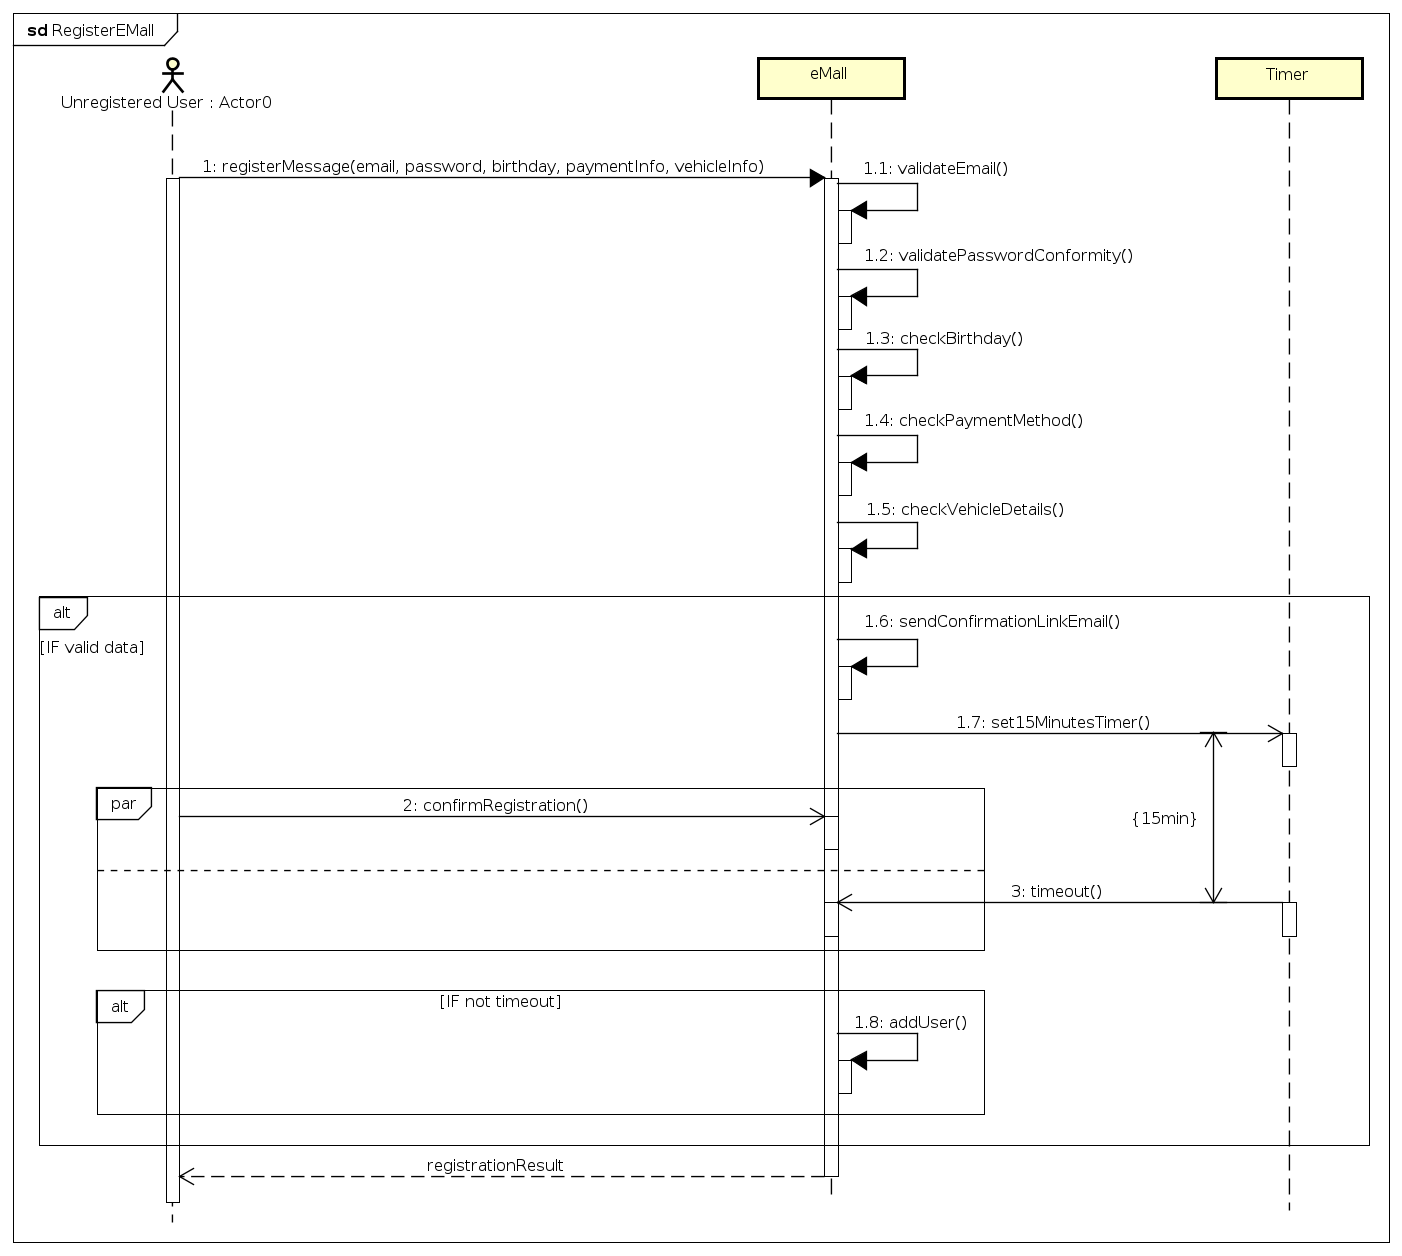
\includegraphics[keepaspectratio, width=16cm]{Sequence/RegisterEMall.png}
        \caption{Registration into \ac{eMall} sequence}
    \end{center}
\end{figure}
\begin{figure}[!h]
    \begin{center}
        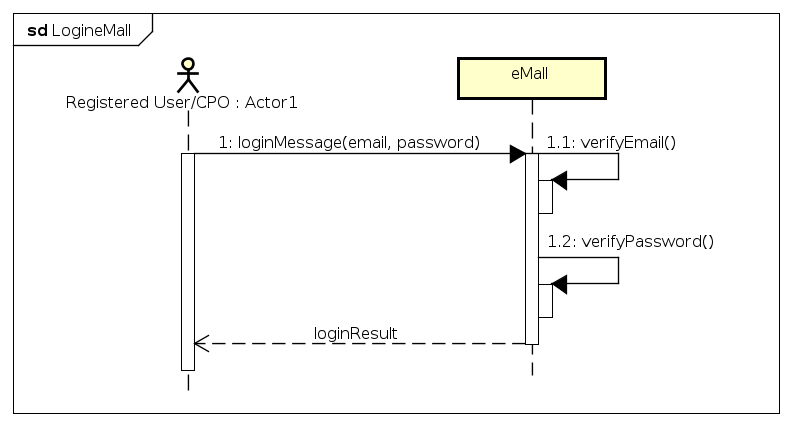
\includegraphics[keepaspectratio, width=16cm]{Sequence/LoginEMall.png}
        \caption{Login into \ac{eMall} sequence}
    \end{center}
\end{figure}
\begin{figure}[!h]
    \begin{center}
        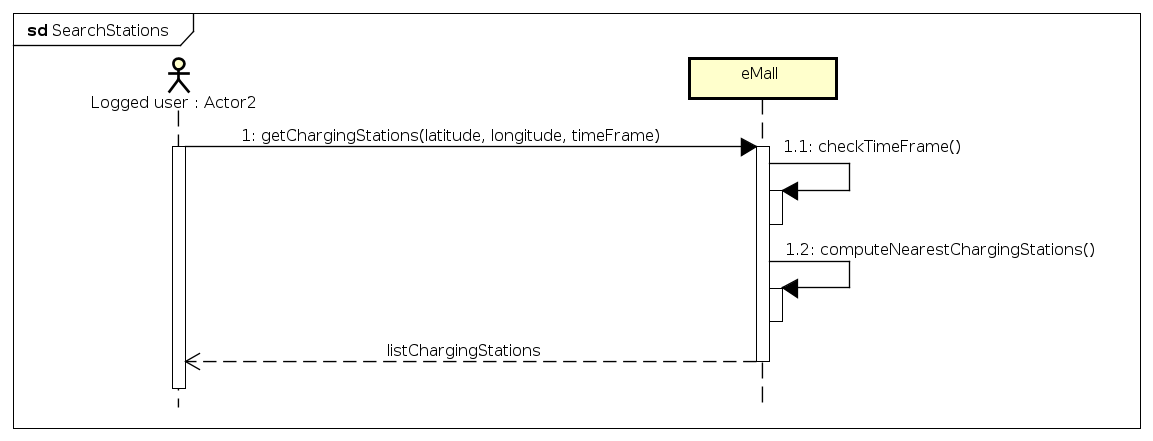
\includegraphics[keepaspectratio, width=16cm]{Sequence/SearchStations.png}
        \caption{Get the nearby charging stations}
    \end{center}
\end{figure}
\begin{figure}[!h]
    \begin{center}
        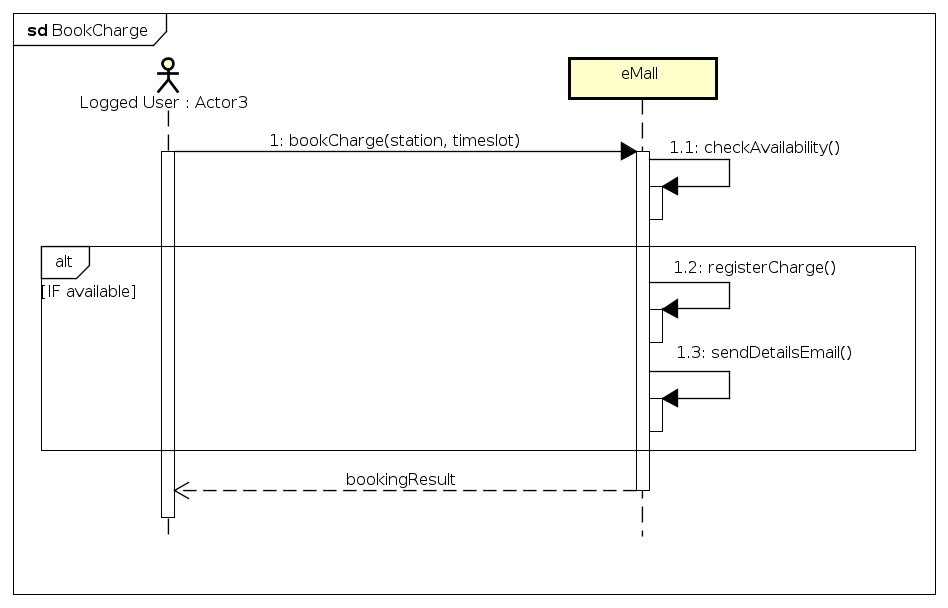
\includegraphics[keepaspectratio, width=16cm]{Sequence/BookCharge.png}
        \caption{Book a charge sequence}
    \end{center}
\end{figure}
\begin{figure}[!h]
    \begin{center}
        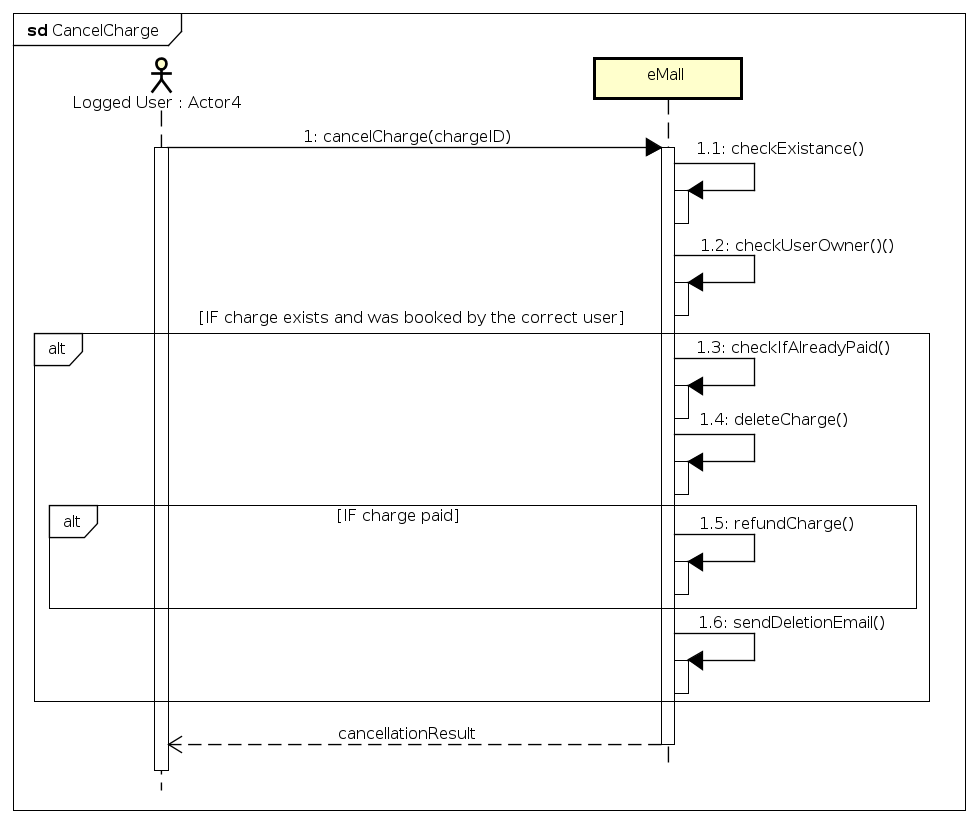
\includegraphics[keepaspectratio, width=16cm]{Sequence/CancelCharge.png}
        \caption{Cancel a charge sequence}
    \end{center}
\end{figure}
\begin{figure}[!h]
    \begin{center}
        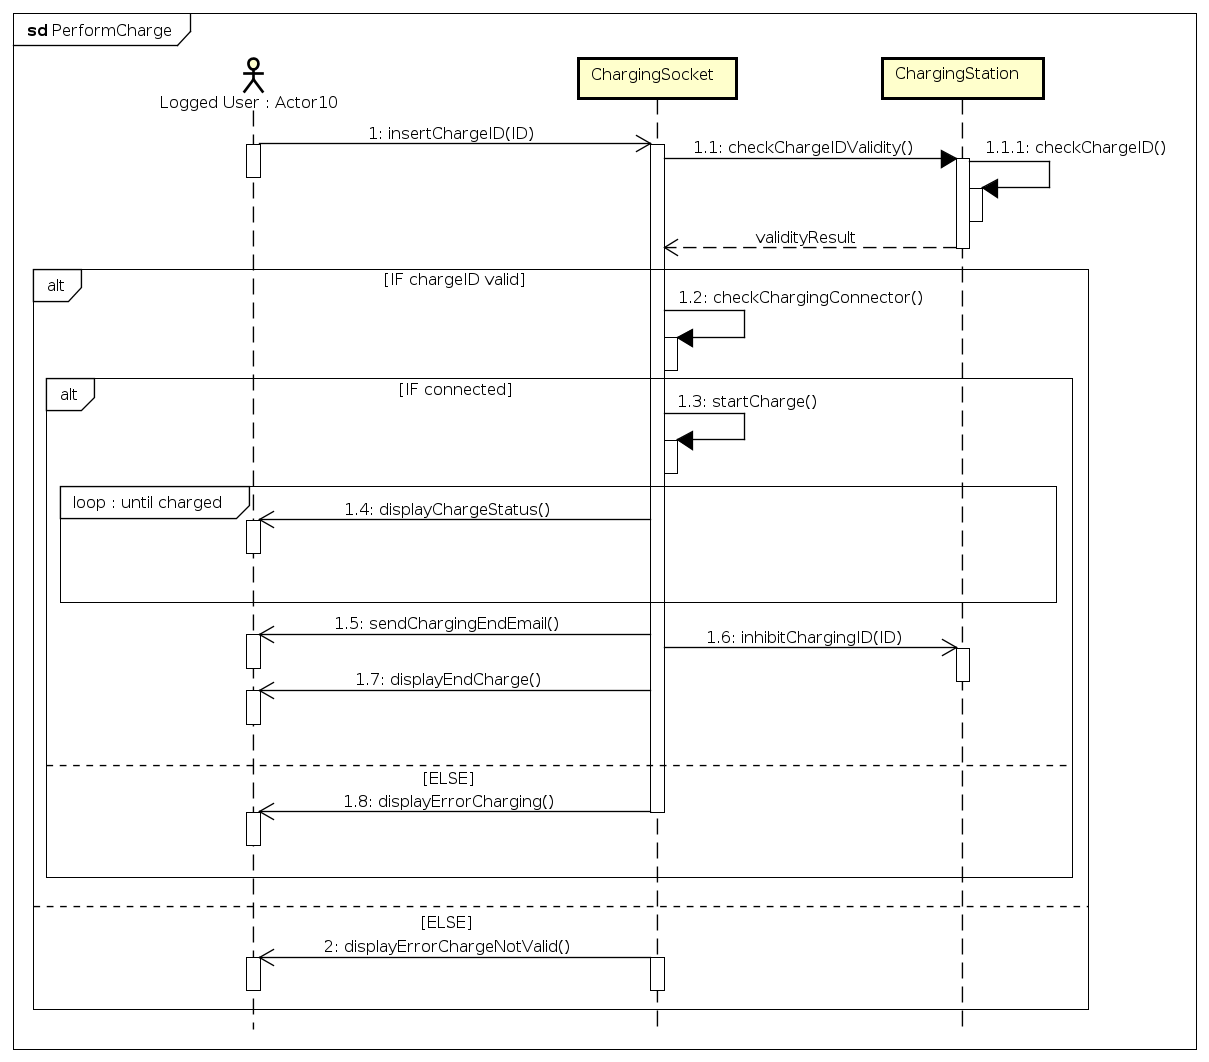
\includegraphics[keepaspectratio, width=16cm]{Sequence/PerformCharge.png}
        \caption{Perform a charge sequence}
    \end{center}
\end{figure}
\begin{figure}[!h]
    \begin{center}
        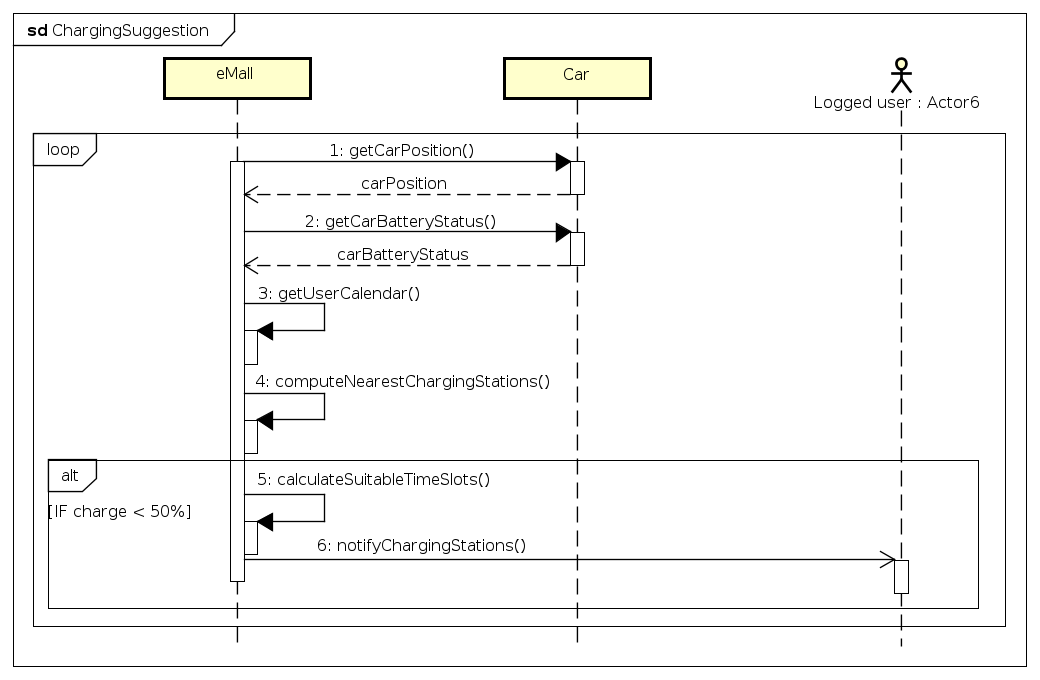
\includegraphics[keepaspectratio, width=16cm]{Sequence/ChargingSuggestion.png}
        \caption{Charging suggestions via calendar sequence}
    \end{center}
\end{figure}

\clearpage
%Definition of use case diagrams, use cases and associated sequence/activity diagrams, and mapping on requirements
\subsection{Performance requirements}
The system in general needs to manage a large collection of electric car users/\acp{CPO} and it needs to supply the heaviest services (like computing the cheapest nearest stations) in a reasonable amount of time.
Because of that the system shall guarantee a baseline load of 1000000 users/\acp{CPO} still with a response time not greater than 5 seconds. To achieve the goal, the system shall be able to decentralize all the computation as possible,
trying to make the client responsible of the heaviest loads.
\subsection{Design constraints}
\subsubsection{Standards compliance}
The system must meet the following standards:
\begin{itemize}
    \item \textbf{GPDR law}: The system must be compliant with the current GDPR law about users privacy;
    \item \textbf{Android and iOS}: The system must be compatible with the current versions and reasonably still used previous ones of Android and iOS.
\end{itemize}
\subsubsection{Hardware limitations}
Because the system consists of a smartphone app, the main hardware limitation is the computational capability of a smartphone processor. Hence the
application must be compatible with a low computational capability.
\subsubsection{Other constraints (TODO MAYBE)}

\subsection{Software system attributes}
\subsubsection{Reliability}
\subsubsection{Availability}
\subsubsection{Security}
\subsubsection{Maintainability}
\subsubsection{Portability}
\subsection{Requirements}
\subsubsection{External Interface Requirements}
\clearpage